\section{Higher-dimensional automata}
\label{sec:higher-dimensional-automata}

    The generalization of independence to $n$ events has lead to a geometric model for concurrency, studied by Pratt and van Glabbeek \cite{pratt91hda, Pratt00Sculptures, Glabbeek06HDA}. Pratt named this model Higher-Dimensional Automata (HDA) \cite{pratt91hda}. With higher-dimensional automata we can distinguish between the execution of $n$ non-interleaving concurrent events and of $n$ mutually exclusive events. Higher-dimensional automata are considered to be of high expressive power because of their property to distinguish $n$-events \cite{Kahl2013TheHG}. Hence, providing a generalization of differences, and common features, of various other models of concurrency, as done in \cite{Glabbeek06HDA} and \cite{Goubault18RelationshipsModelsForConcurrency}. Higher-dimensional automata also retain the state-based view and model the interleaving square with its interior filled, shown in Figure \ref{fig:HDA-filled-interleaving-square}. 
    
   A higher-dimensional automaton is a precubical set that encodes the independence of events by \emph{mappings}. Intuitively, we may consider a precubical set as $n$-dimensional cubes \cite{Fajstrup16DirectedAlgebraicTopologyConcurrency} together with their faces $-$ each $n$-dimensional cube has $2n$ faces. In other words, a front and a back face in each direction $i$ with $0 \leq i < n$. Mappings are families of functions that identify these faces, we call these \emph{face maps}. Face maps that satisfy the \emph{precubical identity} \cite{Fahrenberg05PhD, Fajstrup05DipathsInCubicalComplex, Fajstrup06AlgebraicTopologyConcurrency, Goubault2001TopologicalDeformHDA, goubault2003SomeGeometricPerspectives} are able to interpret the independence of events. In the concurrency theory literature, we find that the precubical identity is named the \emph{cubical law} \cite{Glabbeek06HDA, Johansen16STstruct}, since applications of algebraic topology are still being investigated in concurrency theory. Here, we will follow the topological notion, and use the naming precubical identity.

    Intuitively, the precubical identity is considered to be the idea of "\emph{filling in holes}" of a $n$-dimensional cube \cite[Section 2]{pratt91hda}. This notion is shown in Figure \ref{fig:HDA-filled-interleaving-square}, where the interior of the interleaving square is filled. With higher-dimensional automata we are able to capture the main characteristic of both transition systems and asynchronous transition systems by the notion of "\emph{filling in holes}".
    
  
    \begin{definition}[Precubical set]
        \label{def:precubical-set}
         A \emph{precubical set} is a graded set $\mathcal{X}= \bigcup_{ n\in \Nat} \mathcal{X}_n$, with $\mathcal{X}_n\cap \mathcal{X}_m= \emptyset$ for $n\ne m$, together with mappings $s_{ k, n}, t_{ k, n}:\mathcal{X}_n\to \mathcal{X}_{ n- 1}$, with $1\leq k\leq n$, satisfying the \emph{precubical identities}
         
         %$\delta_{ k, n}^\nu:\mathcal{X}_n\to \mathcal{X}_{ n- 1}$, $k = 1,\dots, n$, $\nu \in \{0, 1\}$, satisfying the \emph{precubical identity}
        
        \begin{equation*}
            \alpha_{ k, n- 1} \beta_{ \ell, n}= \beta_{ \ell- 1, n- 1} \alpha_{ k, n} \qquad(1 \leq k< \ell \leq n)
        \end{equation*}
        for $\alpha, \beta\in\{ s, t\}$.
    \end{definition}
    
    A \emph{graded} set is a \emph{family of sets} where its elements are $n$-cells. A \emph{family of sets} is the disjoint union of these $n$-cells, $\mathcal{X}_n\cap \mathcal{X}_m= \emptyset$ for $n\ne m$. In the beginning of this Section, we called these $n$-cells for $n$-dimensional cubes. The naming $n$-dimensional cubes comes from Fajstrup et al. \cite{Fajstrup16DirectedAlgebraicTopologyConcurrency}, where $n$-dimensional cubes are precubical sets together with their faces. In this thesis, we will call elements of $\mathcal{X}_n$ for $n$-cells,  or simply cells, even though there are different names for these elements such as \emph{$n$-dimensional cubes} \cite{Pratt00Sculptures, Fajstrup16DirectedAlgebraicTopologyConcurrency}, \emph{$n$-transitions} \cite{Goubault95PhDThesis} and \emph{hypercubes} \cite{Glabbeek06HDA}. If $x \in \mathcal{X}_n$, then we say that $x$ is of dimension $n$ and is written $dim x = n$.
    
    The mappings $s_{ k, n}$ and $t_{ k, n}$  are called \emph{face maps}, and we will usually omit the extra subscript $n$ and simply write $s_k$ and $t_k$. Face maps are families of functions that identify the faces of the $n$-cells, in the same manner as described with $n$-dimensional cubes. Families of functions are usually considered as a set of functions whose equations have a similar form. However, in this context we will interpret them geometrically as faces of a cube.
    
    Each $n$-cell $x \in \mathcal{X}_n$ has \emph{$n$ lower faces $s_1 x,\dotsc, s_n x$} and \emph{$n$ upper faces $t_1 x,\dotsc, t_n x$}, and the precubical identity expresses the fact that ($n-1$)-faces of an $n$-cell meet in common ($n-2$)-faces, see Figure \ref{fig:precubical-set-interleaving-square-preidentity}.
    
    Figure \ref{fig:precubical-set-interleaving-square-geometric} and \ref{fig:precubical-set-interleaving-square-preidentity} represent a 2-cell showing both the four faces $s_1 x$, $t_1 x$, $s_2 x$, $t_2 x$ and the four possible mappings of the precubical identity. Figure \ref{fig:precubical-set-interleaving-square-geometric} is more of a geometrical picture of the 2-cell with its interior filled.
    
    \begin{figure}[ht]
        \centering
        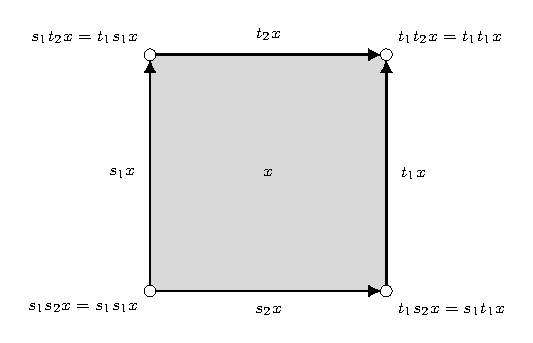
\includegraphics[scale=1.2]{Figures/3.An-introduction-to-non-interleaving-models-for-concurrency/precubical-square/cubical-law-2-cell-geometrical.pdf}
         \captionof{figure}[Geometric representation of a 2-cell]{We have a geometrical picturing of the 2-cell with its interior filled, four faces $s_1 x$, $t_1 x$, $s_2 x$, $t_2 x$ and four corners representing the mappings of the precubical identity.}
        \label{fig:precubical-set-interleaving-square-geometric}
    \end{figure}
    
    While, Figure \ref{fig:precubical-set-interleaving-square-preidentity} shows how the four mappings of the precubical identity is satisfied, and the fact that 1-faces of a 2-cell meet in common 0-faces.
    
    \begin{figure}[ht]
        \centering
        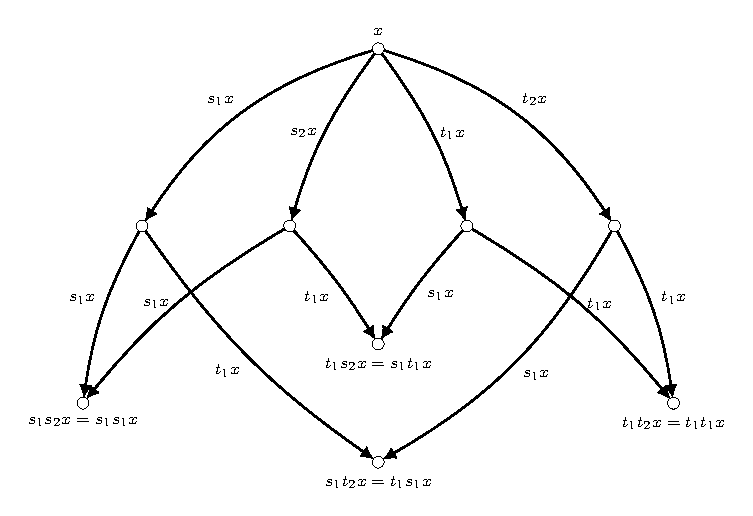
\includegraphics[scale=1]{Figures/3.An-introduction-to-non-interleaving-models-for-concurrency/precubical-square/cubical-law-2-cell-preidentity.pdf}
         \captionof{figure}[2-cell satisfying the precubical identities]{We have a 2-cell showing the four faces $s_1 x$, $t_1 x$, $s_2 x$, $t_2 x$ as edges and the four mappings of the precubical identity as the bottom nodes of the 2-cell.}
        \label{fig:precubical-set-interleaving-square-preidentity}
    \end{figure}
    
    We need a notion of \emph{morphisms} between precubical sets to be able to study the relationship between higher dimensional automata. From Section \ref{sec:ordinary-transition-systems}, we have that morphisms are considered to be simulations. Morphisms as simulation was an idea from Winskel and Nielsen in \cite{winskel95modelsCategory}. We want to extend morphisms to be structure-preserving maps that preserve orientation, shape, and time \cite[Section 2.2]{Goubault95PhDThesis}.
    
    Preserving orientation is addressed by \emph{directed} topology, where the object of study are topological spaces that have a sense of direction. Specifically, a topological space with a directed variant to incorporate the notion of irreversible time. Topology is a branch in mathematics that studies geometric shapes, and directed topology considered these geometric shapes to have a sense of direction. Shapes are preserved if we can present the geometry, we are interested in, as unions of \emph{points, segments, squares, cubes, ..., $n$-dimensional cubes} as collections of \emph{$n$-cells} ($n \in \mathbb{N}$). Preserving time means that we can reason about the directed variant and that every transition is mapped onto a transition.
    
    \begin{definition}[Morphism of precubical sets]
        \label{def:morphism-of-precubical-set}
        Morphisms $f: \mathcal{X}\to \mathcal{Y}$ of precubical sets are graded functions $f=\{ f_n: \mathcal{X}_n\to \mathcal{Y}_n\}_{ n\in \Nat}$ which commute with the face maps:
        
        \begin{equation*}
            \alpha_k\circ f_n= f_{ n- 1}\circ \alpha_k \qquad\ \text{for all}\ n\in \Nat,\ k\in\{ 1,\dots, n\},\ \text{and}\ \alpha\in\{ s, t\}.
        \end{equation*}
    \end{definition}

    Higher-dimensional automata are simply defined in terms of the precubical sets, and the relationship between higher-dimensional automata is described by the morphisms of the underlying precubical sets. Every figure presented thus far, may be considered as a higher-dimensional automata. We will from now on refer to the previous figures as higher-dimensional automata even though we first introduced them as transition systems, asynchronous transition systems and $n$-cells.
    
    \begin{definition}[Higher-dimensional automata \cite{Glabbeek06HDA, Johansen16STstruct}]
        \label{def:higher-dimensional-automata}
        A precubical set $\mathcal{H} = (\mathcal{Q},s,t)$ is a precubical set $\mathcal{Q}$ together with $s$ and $t$ being the collection of all the face maps, that is, for all $n$. 
        
        A higher-dimensional automata is a tuple $(\mathcal{Q}, s, t, l, \mathcal{I}, \mathcal{F})$ over an alphabet $\Sigma$ such that $l(s_i(q)) = l(t_i(q))$ for all $q \in \mathcal{Q}_2$ and $i \in \{1,2\}$, and with a designated initial cell $\mathcal{I} \in \mathcal{Q}_0$ and $\mathcal{F} \subseteq \mathcal{Q}_0$ final cells.

    \end{definition}

    The concurrent execution of a higher-dimensional automata is modeled by including the two-dimensional surface. Intuitively, a concurrent execution can be seen as moving across the surface such that the execution preserves the directed variant, that is, to incorporate a notion of irreversible time. This is pictured in Figure \ref{fig:HDA-filled-interleaving-square}. 
    
    \begin{figure}[ht]
        \centering
        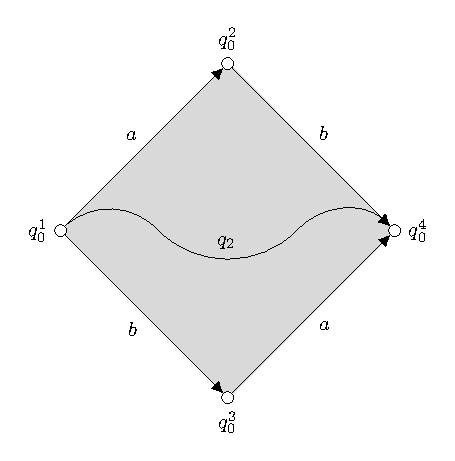
\includegraphics[scale=1.2]{Figures/3.An-introduction-to-non-interleaving-models-for-concurrency/HDA_filled_interleaving_square/filled-interleaving-diamond.pdf}
         \captionof{figure}[Filled interleaving square]{Example of a HDA with four states, $q^1_0, q^2_0, q^3_0$ and $q^4_0$, four transitions, two of which are labeled $a$ and the other two are labeled $b$, and a surface, $q_2$. The surface represents the notion of "filling in holes" \cite[Section 2]{pratt91hda}, which is a continuous deformation of instructions $ab$ into $ba$, or vice versa.}
        \label{fig:HDA-filled-interleaving-square}
    \end{figure}
    
    A computation is a path in this higher-dimensional automaton.
    
    \begin{definition}[Paths in HDAs \cite{Johansen16STstruct}]\label{def_paths_HDA}
        \label{def:paths-in-HDAs}
        A \emph{single step} in a HDA is either
        \begin{enumerate}
            \item $q_{n-1}\transition{s_{i}}q_{n}$ with $s_{i}(q_{n})=q_{n-1}$ or 
            \item $q_{n}\transition{t_{i}}q_{n-1}$ with $t_{i}(q_{n})=q_{n-1}$, 
        \end{enumerate}
        \noindent where $q_{n}\in \mathcal{Q}_{n}$ and $q_{n-1}\in \mathcal{Q}_{n-1}$ and $1\leq i\leq n$. 

        A \emph{path} $\pi\defequal q^{0}\transition{\alpha^{1}}q^{1}\transition{\alpha^{2}}q^{2}\transition{\alpha^{3}}\dots$ is a sequence of single steps $q^{j}\transition{\alpha^{j+1}}q^{j+1}$, with $\alpha^{j}\in\{s,t\}$. We say that $q\in\pi$ iff $q=q^{j}$ appears in one of the steps in $\pi$.  The first cell in a path is denoted $\startPath{\pi}$ and the ending cell in a finite path is $\finishPath{\pi}$. 
    \end{definition}
    
    The markings of the steps by $s$ may be seen as going from a lower cell to a higher cell, and steps by $t$ as the opposite, in the higher dimensional automaton. In many of the later proofs it is though useful to have the exact map easily visible, namely, the index that the step uses, rather than explicitly assuming the index every time. If there is no $\finishPath{\pi}$, then the path is infinite. When the index is not important we write $\transition{s}$ or $\transition{t}$.
    
    \begin{definition}[Histories for $\HDA$s \cite{Johansen16STstruct}]
    \label{def:histories-for-HDA}
    
        In a $\HDA$ two paths are \emph{adjacent}, denoted $\pi\adjacentHDA\pi'$, if one can be obtained from the other by replacing, for $q,q'\in \mathcal{Q}$ and $i<j$,
        
        \begin{enumerate}
            \item a segment $\transition{s_{i}}q\transition{s_{j}}$ by $\transition{s_{j-1}}q'\transition{s_{i}}$, or
            \item a segment $\transition{t_{j}}q\transition{t_{i}}$ by $\transition{t_{i}}q'\transition{t_{j-1}}$, or
            \item a segment $\transition{s_{i}}q\transition{t_{j}}$ by $\transition{t_{j-1}}q'\transition{s_{i}}$, or
            \item a segment $\transition{s_{j}}q\transition{t_{i}}$ by $\transition{t_{i}}q'\transition{s_{j-1}}$.
        \end{enumerate}

        Two finite paths are \textit{l-adjacent} $\pi\ladjacentHDA{l}\pi'$ when the segment replacement happens at position $l+1$; that is, $q$ is the $l+1$ cell in the path. \emph{Homotopy} is the reflexive and transitive closure of adjacency. Two homotopic paths are denoted $\pi\homotopicHDA\pi'$ and share their respective start and end cells. The homotopy class of a rooted path is denoted $\homotopyClass{\pi}$. A homotopy class with end cell $q$ is said to be \emph{a history of $q$}. One cell may have several histories, as is the case with the interleaving square $\HDA$ from Figure~\ref{fig:HDA-filled-interleaving-square}. Whenever a cell has a unique history we use the notation $\homotopyClass{q}$, instead of $\homotopyClass{\pi}$ with $\finishPath{\pi}=q$.
    \end{definition}

    Homotopy is defined for all paths such that a cell of higher dimension has a history in the same way that the inside of a square has a history. The homotopy is provided by Johansen in \cite{Johansen16STstruct}, where the homotopy is different compared to the definition in \cite[Section 1.6]{Goubault18RelationshipsModelsForConcurrency} because not only the state cells of dimension $0$, that is, vertices that form the corners of a cube, have histories, but also cells of higher dimensions.
    
    History unfoldings of process graphs have been defined by Van Glabbeek in \cite[Section 3]{Glabbeek96HistoryUnfolding}. Inspired by the definition of history unfoldings of process graphs, we will define the same notion for higher-dimensional automata. Johansen in \cite{Johansen16STstruct}, provides a definition of history unfolding for higher-dimensional automata which can be correlated with the definition of unfoldings from \cite{Glabbeek96HistoryUnfolding}. Also, alternative definitions of unfoldings for $\HDA$ can be found in \cite{Fahrenberg05PhD, Fahrenberg15PartialHDA}.

    \begin{definition}[History unfolding for HDAs]\label{def_unfolding_history} 
        The \emph{history unfolding} of a higher dimensional automaton $\mathcal{H}$ is a $\HDA$ denoted $\unfolding(\mathcal{H})$, respecting the cubical laws, as shown in \cite[Proposition 3.30]{Johansen16STstruct}, and given by:
        
        \begin{itemize}
            \item $Q_{n}^{\unfolding(\mathcal{H})}$ is the set of histories that end up in cells on level $Q_n$ of $\mathcal{H}$;
            \item has the labelling copied from $\mathcal{H}$: $l^{\unfolding(\mathcal{H})}(\homotopyClass{\pi})=l^{H}(\finishPath{\pi})$;
            \item initial cell the empty rooted history;
            \item the $s/t$ maps are built from the corresponding maps between the end cells of the histories: 
                \[
                    s_{i}(\homotopyClass{\pi})=\homotopyClass{\pi'}\mbox{\ \ \ iff\ \ \ }s_{i}(q)=q'\wedge \pi'\transition{s_{i}}\pi\wedge \finishPath{\pi'}=q'\wedge \finishPath{\pi}=q;
                \]
                \[
                    t_{i}(\homotopyClass{\pi})=\homotopyClass{\pi'} \mbox{\ \ \ iff\ \ \ } t_{i}(q)=q' \wedge \pi\transition{t_{i}}\pi' \wedge \finishPath{\pi'}=q'\wedge \finishPath{\pi}=q.
                \]
        \end{itemize}
    \end{definition}
    
    The notion of \emph{unfolding} removes iteration and is commonly used to turn a complicated model such as higher-dimensional automata into a simpler, but potentially infinite one. Unfolding is important in relation to the sculpting method introduced in Chapter \ref{chap:sculpting-in-concurrency}. For HDA this picture is more complicated.  Figure~\ref{fig:HDA-broken-box} (left) shows a simple HDA which is a sculpture. However, we will show that its unfolding (right) is \emph{not} a sculpture.

    \begin{definition}[Morphism of HDAs \cite{Johansen16STstruct}]
        \label{def:isomorphism-of-higher-dimensional-automata}
        A morphism between two \emph{HDA}s, $f : \mathcal{H} \rightarrow \mathcal{H}'$ is a dimension preserving map between their cells $f : \mathcal{Q} \rightarrow \mathcal{Q}'$, such that:
        
        \begin{enumerate}
            \item the initial cell is preserved: $f(\mathcal{I}) = \mathcal{I}'$
            \item the labelling is preserved: $l'(f(q_1)) = l(q_1)$ for all $q_1 \in \mathcal{Q}_1$,
            \item the mappings are preserved, for any $q_n \in \mathcal{Q}_n$ and $1 \leq i \leq n$:
            \begin{itemize}
                \item $s'_i(f(q_n)) = f(s_i(q_n))$ and
                \item $t'_i(f(q_n)) = f(t_i(q_n))$.
            \end{itemize}
        \end{enumerate}
        
        When a morphism is bijective we call it isomorphism. Two HDAs are isomorphic, denoted $\mathcal{H} \cong \mathcal{H}'$, when there exists an isomorphism between them.
    \end{definition}

    We write $\allHDA$ for the category of higher-dimensional automata, where the object of the category are higher-dimensional automata and morphisms are as defined in Definition \ref{def:isomorphism-of-higher-dimensional-automata}.
    
    In the definition of precubical sets, we consider them to be non-degenerate. Many of the results from this thesis assumes higher-dimensional automata to be non-degenerate. Also, we consider the directed variant, mentioned so far, to be higher-dimensional automata that are acyclic. Johansen in \cite{Johansen16STstruct}, defines these notions for higher dimensional automata:
    
    \begin{definition}[Acyclic and non-degnerate HDAs \cite{Johansen16STstruct}]
        \label{def:acyclic-and-non-degenerate-higher-dimensional-automata}
        A higher-dimensional automata is called acyclic if no path visits a cell twice. A higher-dimensional automata is non-degenerate if for any cell $q$ all its faces exist and are different, in the sense of $\forall i \neq j : \alpha_i(q) \neq \beta_i(q) \wedge \alpha , \beta \{s,t\}$, no two transitions with the same label share both their end states.
    \end{definition}
    
    The notion of acyclic does not allow cycles, or loops, in the higher-dimensional automata, and the notion of non-degeneracies is related to the underlying precubical sets\footnote{In topology, The distinction between non-degeneracies and degeneracies are subtle and will not be considered here. In \cite{Goubault95PhDThesis}, the  distinction between non-degeneracies and degeneracies is considered.}. The restriction on higher-dimensional automata being non-degenerate is similar to that of Fajstrup et al. \cite{Fajstrup16DirectedAlgebraicTopologyConcurrency} and that of van Glabbeek \cite{Glabbeek06HDA}. Also, the restriction above is the same for precubical sets where two opposite s-maps and t-maps can be equal, such that $s_i(q) = t_i(q)$ is allowed. We assume all s-maps and t-maps are to be total, as done in \cite{Johansen16STstruct}. A study of partial higher-dimensional automata, where s-maps and t-maps are partial, has been considered by Fahrenberg in \cite{Fahrenberg15PartialHDA}.